\subsection{Motivation} \label{sec:body_motivation}

The world record in recalling historic dates is roughly equal to all the dates children have to learn during their entire time in school. The world record holder did it in five minutes while the average high-school student, looking back on their 12 years of education, is likely to remember no more than a handful of them \cite{how_to_become_a_memory_master}. It took Zou Lujian 13.96 seconds to remember the order of a shuffled deck of 52 playing cards \cite{record_recall_playing_cards}. When people are presented with these achievements they often assume only extremely rare geniuses could accomplish such tasks or perhaps think that aliens really are among us. To me that highlights a lack of awareness of the surprisingly simple techniques that are being used by all of these aliens. It also emphasizes how little we trust our ability to remember. "If you don't know the information is there, you don't trust your brain. If you don't trust your brain you study all the time."\cite{how_to_become_a_memory_master}. This quote reminds me of the distress I've felt before taking exams that involved a lot of memorization during my time in school. I've heard of people puking before medical exams and it is not surprising to me when I think of my sister's condition before she had her preliminary medical exam. I'm sure people can relate to this. Following what techniques enable the average person to trust their brain and if they are so simple and effective why are they not ubiquitous? We call those techniques \emph{mnemonics} and their usage dates back far beyond the Ancient Greeks \cite{white_2014}. Simonides allegedly helped to identify bodies of a collapsed building as he had remembered every person in a large banquet hall of the building by using a mnemonic device that we call today \emph{loci}. As the word loci suggests, it works by imagining a familiar place in one's mind and associating parts of that place with words from e.g. a shopping list or in the rather peculiar example of Simonides, a group of people. If your're list requires ordering you can use the \emph{peg system} where you first must memorize a list of distinct objects after which you could associate each item on the list with e.g. the first 10 presidents of the US. If there is a mnemonic device that is known to almost everyone, it is probably \emph{acronyms}. You may use or have used \emph{soh cah toa} to remember ratio formulas of triangles. Although these methods may already inspire curiosity in the field, it's quite a leap to think that people can remember up to 70000 decimal places of \emph{pi} by using them \cite{record_decimal_pi}. Alongside an insatiable desire to learn things that are arguably useless, except for impressing the public, there must be another layer that closes the gap between techniques described so far and remembering inherently abstract things like numbers. This can be achieved by using \emph{phonetic systems}. The method utilizes a table that maps numbers to consonants that can then be employed to form words. The word \emph{cup} for instance translates to the number \emph{79} with the so called \emph{major system} \cite{major_system}. Subsequently you turn numbers into words and words into stories to remember the entire sequence. While this may be used to recall the number of your close ones the next time you are lost in the wild without a phone, with enough practice, you may start having aspirations to break the record in recalling decimal places of pi. Another common technique is the \emph{keyword mnemonic} that steps out of the memory athlete realm and shines with more practical applications most commonly found in second language learning. The process involves finding a keyword that is phonetically similar to the one the student wants or perhaps more accurately is obliged to learn and then form a sentence or phrase that connects the two words in a meaningful manner. E.g. the Japanese word 食べる (taberu) meaning \emph{to eat} sounds like the word \emph{table}. Following one could come up with a phrase like so: "Imagine you eat your lunch on the table. You wouldn't eat on the floor. That's inappropriate!". It seems only natural to assume that given their incredible success among memory athletes mnemonic devices should be everywhere in education. Evidently they are almost nowhere in traditional education except for a few acronyms here and there. To unwrap that conundrum it is worth looking into existing research on the topic. Most of the research I have come across tests the effectiveness of mnemonics in education by comparing groups that use mnemonics with groups that do "nothing", or at least do nothing special to recall the given material. Because of it's application in second language learning keyword mnemonics are a common choice for these comparisons. Participants are usually shown a list of foreign words to remember and later asked to recall them at different time intervals. Ample such studies suggest that the use of mnemonics in education significantly improves academic performance while others do not \cite{putnam_2015}. This may be due to the simplistic nature of conducted studies as they often neglect the fact that the control group is already using mnemonic devices, whether participants are aware of it or not, as has been shown by \cite{the_do_nothing_group} explaining \emph{what the "do-nothing" group does}. Additionally mnemonic devices have been criticized to be no better than more straightforward methods like repetition and taking notes when it comes to long-term learning \cite{putnam_2015}. To assume that there exists a learning method that lets individuals engrave information into their brain like a read/write head does on a hard disk is preposterous. It is important to note that mnemonics can enhance learning but still require repetition. Furthermore I argue that mnemonics are a much more engaging and fun way of learning and given that groups utilizing mnemonics almost always outperform the control groups in immediate retrieval \cite{putnam_2015} of the learned material, I find it reasonable to suggest that learning with mnemonics also saves time. Most importantly mnemonics can help individuals to regain trust in their brain's ability to recall information which also reduces anxiety in students as they have a sort of legal "cheat sheet" during exams \cite{putnam_2015}. Despite my appraisal of mnemonic devices they are still not found very often in the classroom or the everyday life. It's not very difficult to see the reason for the latter as we no longer have to rely on our brains to remember as much. White has pointed out that with Gutenberg's invention of the printing press mnemonic devices were swept off the table as information was now much more accessible. \cite{white_2014} The revolution that came with digital information and the internet of course only accelerated this development. And while using mnemonics to remember phone numbers of your close ones seemed very useful 20 years ago, the need for this has been virtually eradicated with modern smartphones.

I believe the lack of mnemonics in the classroom is due to the fact that using them seems to involve extra work or initial efforts like memorizing a peg list or finding an appropriate keyword. This in turn makes them rather unattractive for already unmotivated students.
I believe the latest developments in Artificial Intelligence can bring mnemonics back into the classroom. \emph{ChatGPT} has made the recent progress of large language models like \emph{GPT-3} accessible to the average person and their potential to use mnemonics more effectively is inexhaustible. However I focus my work on the specific use case of learning Japanese \emph{Kanji}. Websites like \emph{Wanikani} \cite{wanikani} have been successful in teaching students Kanji with mnemonics. \emph{Radicals} are components that make up Kanjis and when you combine their meanings with the meaning of the Kanji at hand you can create a mnemonic story or expression that combines the meanings from the Kanji and its Radicals. Figure \ref{figure:robanohashi_example} shows an example of this from the application I have built in conjunction with this paper.
\begin{figure}
    \centering
    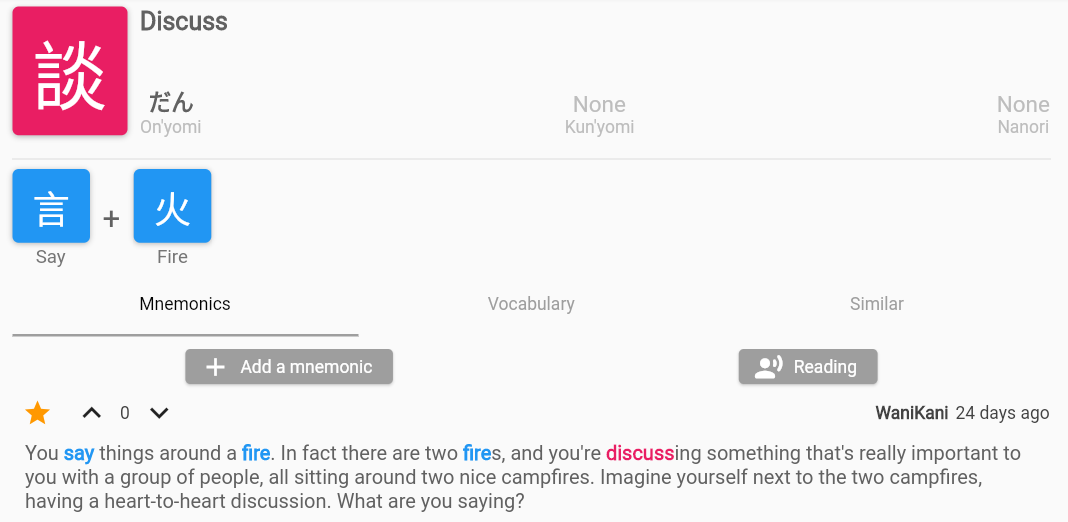
\includegraphics[width=400pt]{resources/robanohashi_example.png}
    \caption{This is a screenshot of \emph{robanohashi.org} show casing the mnemonic device used for learning Japanese Kanji}
    \label{figure:robanohashi_example}
\end{figure}
I suspect that thanks to the provided, handcrafted mnemonics from Wanikani the site has been a success and is backed by a strong community. Having to create the mnemonics by hand they limited themselves to only the common Kanjis and words. With the power of language models we can now extend this database of mnemonics and also enrich it as the effectiveness of mnemonics also depends on the individual because certain mnemonics are more relatable than others, depending on personal experiences. Once you generate a few mnemonics you quickly run into a dead end when trying to evaluate the output. Hence I find it important to discriminate the quality of different outputs not only to find the optimal prompts but perhaps also to uncover linguistic features that capture the effectiveness of mnemonics, as research on this limited. 



